\renewcommand{\chaptername}{Chapter} 
\chapter{Joint estimation of perseveration and reverse correlation parameters with GLM-HMM model}\label{chap7}
As discussed in Chapter \ref{chap5}, kernel estimation using normative models like Weighted Sums and Generalized Linear Models (GLMs) does not fully account for perseveration behavior in stroke patients. This behavioral bias reduces the precision of kernel estimation in these models. 
One of the puzzling aspects of kernel estimation in perseverating observers is that despite using models designed to capture stimulus-response relationships, the true underlying decision process remains obscured. For instance  an observer with a low probability of staying in the perseverative state $p_{perseveration}=0.05$ achieves a high correlation $\rho=0.8$ between the estimated and true kernel. In contrast, a highly perseverative observer $p_{perseveration}=0.95$ exhibits a reduced correlation $\rho=0.45$, indicating a greater deviation from the true kernel.
Our initial approach to detecting perseveration in behavioral responses relied solely on choice history, measuring the perseveration ratio—the tendency to repeat the same response across consecutive trials—without considering whether the response was appropriate to the stimulus. However, perseveration is also a known symptom of aprosodia after stroke. Detecting it provides crucial insights into the behavioral traits of patients, potentially offering a better understanding of their cognitive impairments. This chapter aims to move beyond single-state models and demonstrate how to extract two distinct cognitive states in response to a reverse correlation experiment.
%$Normative models assume that the observer responds identically on every trial, ignoring potential internal state fluctuations. However, behavior is often driven by latent states, which influence decision-making over time.  


\section {Discrete latent states underlying human decision-making}
The assumption of a single-state decision process fails to capture the dynamical nature of human behavior. Instead, we can reframe the problem as a dynamical system using State-Space Models (SSMs) a partially observed Markov model, providing a framework for modeling hidden cognitive states that evolve dynamically. SSMs have been applied, from their early use in the 1960s Kalman filter for spacecraft tracking, to their application in animal movement modeling (1990s), and later in complex behavioral models (2013) for capturing hidden cognitive and decision-making processes.
At their core, SSMs consist of two modeling part: (1)The Process Model – Captures how the system evolves over time.  (2) The Observation Model – Maps observations to hidden states, accounting for measurement noise and indirect observations.By decoupling these components, SSMs effectively handle observational errors and reveal latent cognitive dynamics, making them particularly useful for behavioral and neural modeling.

\subsection{HMM}

The process model in SSM  can be a Hidden markov models (HMMs) in which the system being modeled is assumed to be a Markov process with discrete (i.e. hidden) states $z_{t}$. In probability theory, a Markov model is a stochastic model used to model randomly changing systems. It is assumed that future states depend only on the current state, not on the events that occurred before it.
The observations may be discrete, $y_{t}\in \{1, 2, \dots, N_{y}\}$, or continuous and assumed to be generated from these latent states. 
An HMM consists of: 
\begin{itemize}
    \item The initial state distribution $p(z_{1}=i)=\pi_{i} $.
    \item The transtiton model is noted as $p(z_{t}=j|z_{t-1}=i)=A_{ij} $ which shows how likely to change from one latent state $i$ to $j$, the diagonal of this matrix shows the percentage of staying on one state or stickiness.
    \item The observation model has emission probabilities as $p(y_{t}|z_{t}=j) $ which specifies how observations $y_{t}$ are generated given the latent state $z_{t}$ .
For continuous observations, a Gaussian emission model is often used:  $p(y_{t}|z_{t}=j) = N(y_{t}; \mu_{j},\sigma^2_{j})$ . 
\end{itemize}
Since latent states are not directly observable, parameter estimation is performed using the Expectation-Maximization (EM) algorithm, specifically the Baum-Welch algorithm, which iteratively refines the model parameters , which alternates between two steps:
\begin{itemize}
    \item E-step: We estimate the probability of being in each hidden state at every point in time based on the observations. This is done using the Forward-Backward Algorithm, which calculates the posterior probabilities of hidden states (probability distribution over the hidden states at a given time, given the entire sequence of observed data up to that point).
    \item M-step: Using these probabilities, updates the model’s parameters, including the transition matrix (how hidden states change over time) and the emission parameters (how hidden states affect the observations). The goal is to maximize the likelihood of the observed data.
\end{itemize}

\subsection{IO-HMM}
Input-Output HMM (IO-HMM) first introduced by Bengio and Frasconi in 1995, extends the HMM by allowing external inputs $x_{t}$ to influence both latent state transitions and emissions.  unlike standard HMMs, which the distributions of the output variables  are conditioned solely  on the states . The transition model is  input-dependent in IO-HMM $p(z_{t}=j|z_{t-1}=i,x_{t})$
and the observation model is also conditioned on $x_{t}$: $p(y_{t}|z_{t}=j,x_{t}) $. This modification allows latent state changes to be influenced by contextual information, making IO-HMMs more flexible for modeling stimulus-driven behaviors. 


\subsection{GLM-HMM}
The Generalized Linear Model Hidden Markov Model (GLM-HMM) extends the HMM by incorporating external inputs $x_{t}$ into the observation model, which models observations as a function of both latent states and input-dependent covariates. In the GLM-HMM, the HMM governs the distribution over latent states, while a state-specific GLM specifies the strategy of decision-making within each state. The GLM maps observations $y_{t}$ 
to a weighted combination of covariates (e.g., stimulus, trial history, and bias) through a sigmoidal function, modeling the probability of a binary decision. This formulation allows each latent state to impose a different weighting on the covariates, capturing distinct behavioral strategies.
The probability of a binary response $y_{t}$ in a given latent state $z_{t}$ is defined as:
\begin{align}
p(y_{t}=1|x_{t},z_{t}) &= \frac{1}{1 + e^{-x_{t}.w_{z_{t}}}}=\sigma(x_{t}.w_{z_{t}}).
\end{align}
Unlike IO-HMMs, where latent state transitions are input-dependent, in GLM-HMMs, transitions remain Markovian, while the observations $y_{t}$ depend on both latent states $z_{t}$ and external inputs $x_{t}$ making the GLM-HMM particularly useful for modeling state-dependent decision-making processes.  

\section{Training Algorithm for GLM-HMM}

As the theoretical overview, the parameters of the GLM-HMM are estimated using the Expectation-Maximization (EM) algorithm. EM iteratively optimizes the parameters by alternating between computing posterior probabilities of latent states E-step and updating model parameters M-step. Depending on the estimation method, we can use either Maximum Likelihood Estimation (MLE) or Maximum A Posteriori (MAP) Estimation.
\subsection{Maximum Likelihood (MLE) Estimation }

MLE estimates the parameters by maximizing the likelihood of the observed data:

\begin{align}
\hat{\Theta} = \arg\max_{\Theta} P(y_{1:T} | x_{1:T}, \Theta)
\end{align}

where \( \hat{\Theta} \) represents the optimal parameter estimates based purely on observed data.
Since the latent states  are unobserved, the EM algorithm is used to iteratively refine the model parameters. It consists of two steps: 

E-Step: Compute Posterior Probabilities: Using the Forward-Backward algorithm, we compute the posterior probability of each latent state:

\begin{align}
\gamma_{t,k} &= P(z_t = k | y_{1:T}, x_{1:T}, \Theta)
\end{align}

where $\gamma_{t,k}$ epresents the probability of being in latent state k at time , entire sequence of observations and inputs.

Additionally, we compute the expected state transitions:

\begin{align}
\xi_{t,ij} &= P(z_t = i, z_{t+1} = j | y_{1:T}, x_{1:T}, \Theta)
\end{align}

which represents the probability of transitioning from state \( i \) to state \( j \).
M-Step: Update Model Parameters

Using the posterior estimates from the E-Step, we update the model parameters by maximizing the expected log-likelihood.
The transition matrix \( A \) is updated as:

\begin{align}
A_{ij} &= \frac{\sum_{t=1}^{T-1} \xi_{t,ij}}{\sum_{t=1}^{T-1} \gamma_{t,i}}
\end{align}

ensuring that transitions remain valid and sum to one.

The GLM parameters \( w_k \) are updated by maximizing the conditional log-likelihood:

\begin{align}
\max_w \sum_{t=1}^{T} \sum_{k=1}^{K} \gamma_{t,k} \log P(y_t | x_t, w_k)
\end{align}

which is typically optimized using gradient ascent.

\subsection{Maximum A Posteriori (MAP) Estimation} 


MAP extends MLE by incorporating prior distributions on the model parameters to regularize estimation. It maximizes the posterior probability:

\begin{align}
\hat{\Theta} = \arg\max_{\Theta} P(y_{1:T} | x_{1:T}, \Theta) P(\Theta)
\end{align}

where \( P(\Theta) \) represents the prior distribution. This ensures that the estimated parameters remain within reasonable ranges, especially when data are limited.

MAP follows the same EM procedure as MLE, but with additional regularization from prior distributions. 
As in MLE,  in the E-step we compute the posterior probabilities of the latent states, and the expected transition probabilities. What is different here is the M-step, which incorporates prior distributions to regularize parameter updates. 

\begin{itemize}
    \item The transition matrix A is updated similarly to MLE but constrained by a Dirichlet prior which ensures that transition probabilities remain non-negative and sum to one:
    \begin{align}
    P(A) = \text{Dirichlet}(A | \alpha)
    \end{align}
    \item The GLM parameters \( w_{k}\) are updated by maximizing the posterior probability: 
\begin{align}
\max_w \sum_{t=1}^{T} \sum_{k=1}^{K} \gamma_{t,k} \log P(y_t | x_t, w_k)+\log P(w_k)
\end{align} 
\item where the prior $P(w_{k})$ is modeled as a Gaussian distribution:
    \begin{align}
    P(w) = \mathcal{N}(w | \mu, \sigma^2)
    \end{align}
\end{itemize}

MAP estimation is particularly beneficial when the dataset is limited, as it incorporates prior knowledge to improve generalization and prevent overfitting.

\section {Application on perseverating observer} 
This method has already been applied to mice as a descriptive model, demonstrating dynamic switching between an engaged state, where decisions rely on sensory input, and biased states, where errors are more frequent. This study contributed to the development of the SSM (State Space Model) library by Scott Linderman's lab, which I use in my analysis. In \cite{ashwood_mice_2022}, the authors aimed to determine the number of states that best explain movement-based decision-making in mice by minimizing the log-likelihood across subjects. Similar state-space models have been widely used in neuroscience to study movement, motor control, and neural activity, capturing underlying dynamical structures in behavior. Unlike Ashwood et al.2022 study, where state transitions were inferred from known correct responses, we do not have ground truth for state switching or the correct response in the reverse correlation experiment. To overcome this limitation, we use the Palin framework to simulate multiple perseverating observers with known true states, allowing us to validate the switching algorithm.
Our GLM-HMM model takes as inputs the difference in features between manipulated stimuli in each trial and an additional covariate—the observer's previous choice. If an observer’s response at trial\( t \) is identical to their response at trial \( t-1 \), and this choice is not based on the stimulus representation, they are classified in the perseverative state. Conversely, if their choice is influenced by the stimulus, they are classified in the engaged state. Our goal is to determine, for each trial, whether the observer is in the engaged or perseverative state, providing a state-based interpretation of decision-making behavior while drawing parallels with motor control impairments.
\begin{figure}[H]
    \centering
    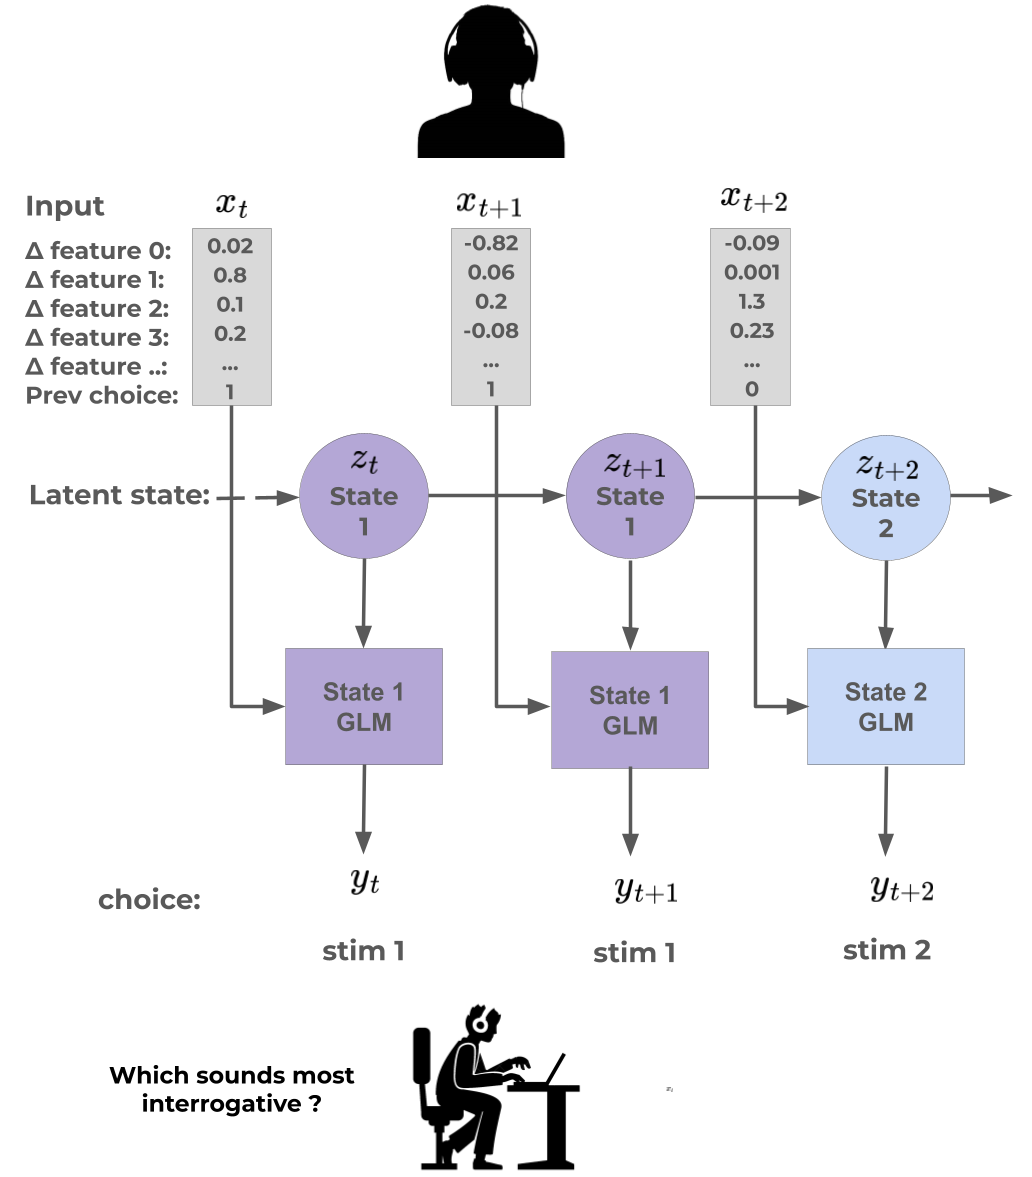
\includegraphics[width=12cm]{MainLayout/Images/chapter7/experiment_model.png}
    \caption{Main Title for First Image \\ \small Subtitle for the first graphic.}
    \label{fig:patient_responses}
\end{figure}


\subsection {Estimation methods-MLE} 
With Maximum Likelihood Estimation (MLE), we consistently observe nonzero weights on choice history in both states because MLE optimizes the likelihood without incorporating prior constraints. Since choice history is often predictive of the current choice, the model naturally assigns weights to this covariate in both states, even when one state (the engaged state) should ideally rely solely on stimulus-driven decision-making. This issue arises because MLE does not enforce state-specific constraints, allowing information from past choices to leak into both states rather than being confined to the perseverative state alone. Additionally, MLE is prone to overfitting, capturing any correlation in the data that increases likelihood, even if it does not reflect the true underlying cognitive states. Without a prior to guide the estimation, the model struggles to separate the engaged and perseverative states properly, leading to a failure in state dissociation. Additionally, MLE only seeks to maximize the likelihood of observed choices, which makes it susceptible to local likelihood optima, where the optimization process gets stuck in suboptimal solutions. This is particularly problematic when the dataset is limited in the number of trials.

\subsection {Estimation methods-MAP} 
To overcome these limitations, Maximum A Posteriori (MAP) estimation is essential, as it allows us to incorporate structured priors that guide the learning process and prevent state ambiguity. To ensure that MAP correctly distinguishes between engaged and perseverative states, we designed a systematic validation approach by simulating multiple perseverating observers in PALIN with a known ground truth of state transitions, to optimize priors for both GLM weights (Gaussian priors) and transition probabilities (Dirichlet priors). Since prior selection significantly influences state recovery, we leveraged Bayesian optimization to explore a broad set of parameter values and identify those that best facilitate the separation of latent states. This controlled setup enabled us to test how well different prior distributions influence model convergence and state recovery.


\begin{figure}[H]
    \centering
    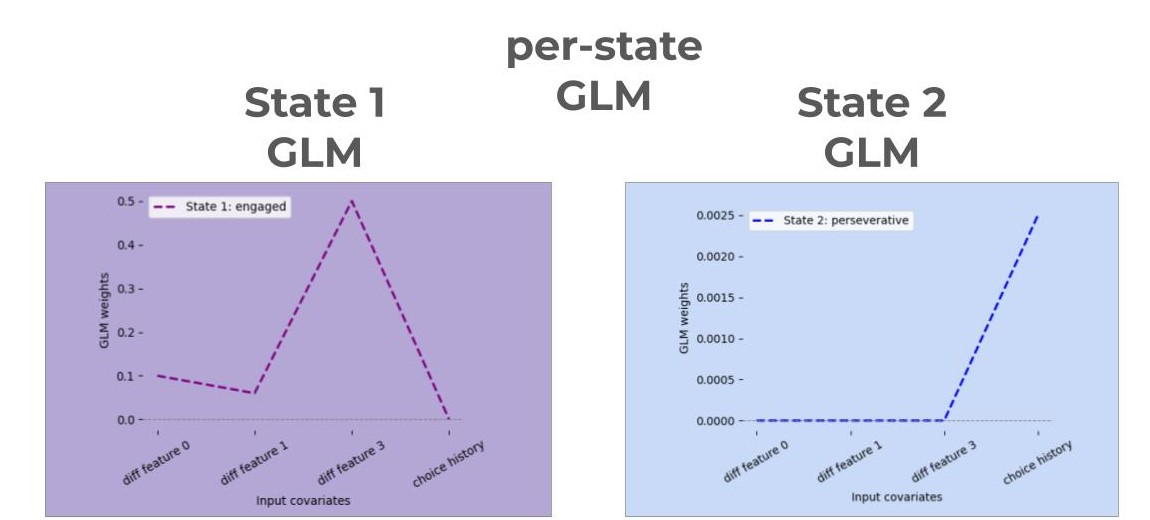
\includegraphics[width=15cm]{MainLayout/Images/chapter7/glm_perstate.jpg}
    \caption{Main Title for First Image \\ \small Subtitle for the first graphic.}
    \label{fig:patient_responses}
\end{figure}
\begin{figure}[H]
    \centering
    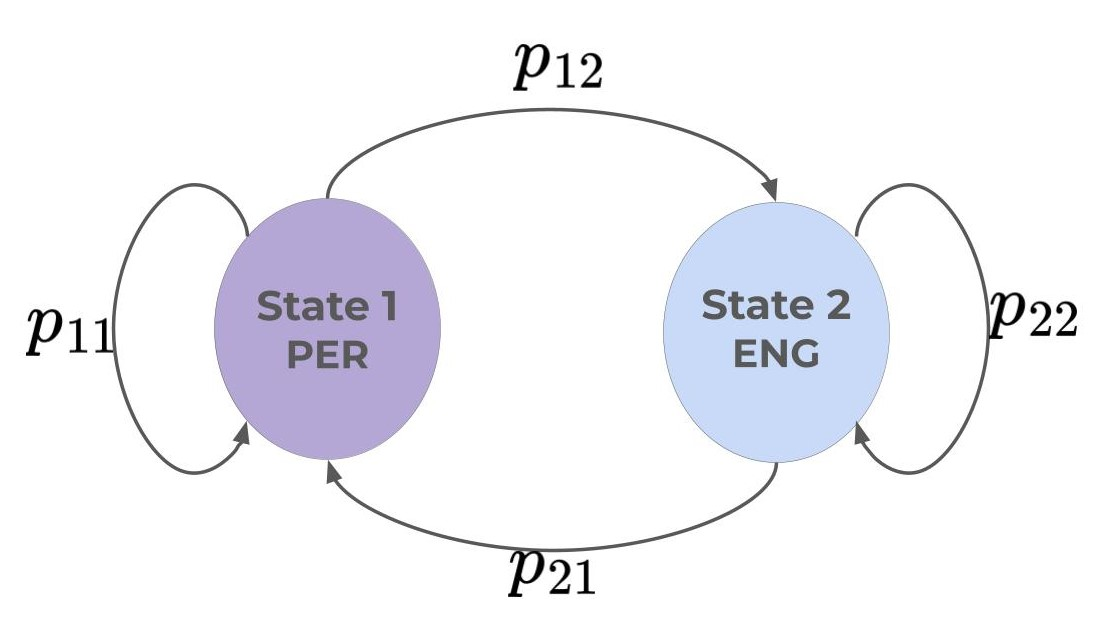
\includegraphics[width=8cm]{MainLayout/Images/chapter7/transition.jpg}
    \caption{Main Title for First Image \\ \small Subtitle for the first graphic.}
    \label{fig:patient_responses}
\end{figure}

\subsubsection{Bayesian Optimization}
We put the model in the condition of real reverse correlation experiment, which was designed with two discrete states, one observed dimension representing responses, and eight input covariates, including stimulus-related features and choice history. The outputs were modeled as binary responses. To refine the prior selection in Bayesian optimization the priors for the GLM weights were defined using gaussian distributions wide range of mean $\mu$ and variance $\sigma^2$, while the transition probabilities were controlled using a dirichlet prior with an adjustable concentration parameter $\alpha$.
\subsubsection{Calculating RMSE}
The posterior state probabilities were computed, and predicted states were compared against the true simulated states to evaluate the accuracy of state recovery. This was assessed through root mean square error (RMSE) measures the difference between true $z$ and predicted latent variables $z$ from the estimators, both in terms of total state recovery and separately for each latent state, and the optimization process selected the priors that minimized RMSE. Additionally, we recorded the log-likelihood of the fitted model to assess its overall fit to the data.
\begin{figure}[H]
    \centering
    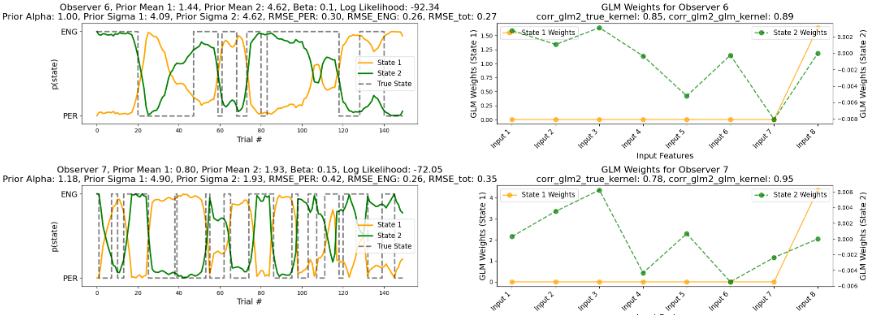
\includegraphics[width=16cm]{MainLayout/Images/chapter7/bo_glmhmm.png}
    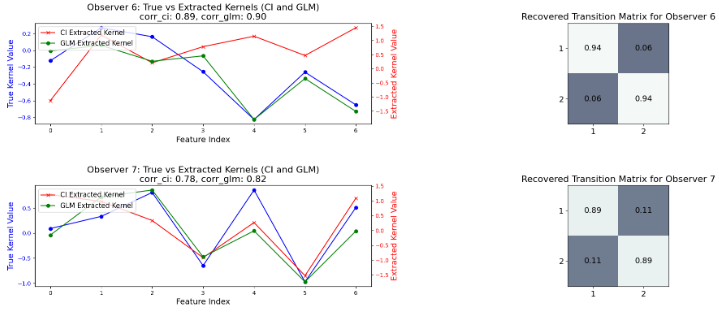
\includegraphics[width=16cm]{MainLayout/Images/chapter7/bo_glmhmm1.png}
    \caption{Main Title for First Image \\ \small Subtitle for the first graphic.}
    \label{fig:patient_responses}
\end{figure}
\section{Validation}
To apply these priors to extract the perseverative state from the responses of stroke patients, we averaged the prios as $\mu$ and variance $\sigma^2$, and $\alpha$, and called them best priors, fit the GLM-HMM with these best priors once to each subject, and we can extract the posterior probability of each trial, the transiton matrix and fitted GLM weights. 
\begin{figure}[H]
    \centering
    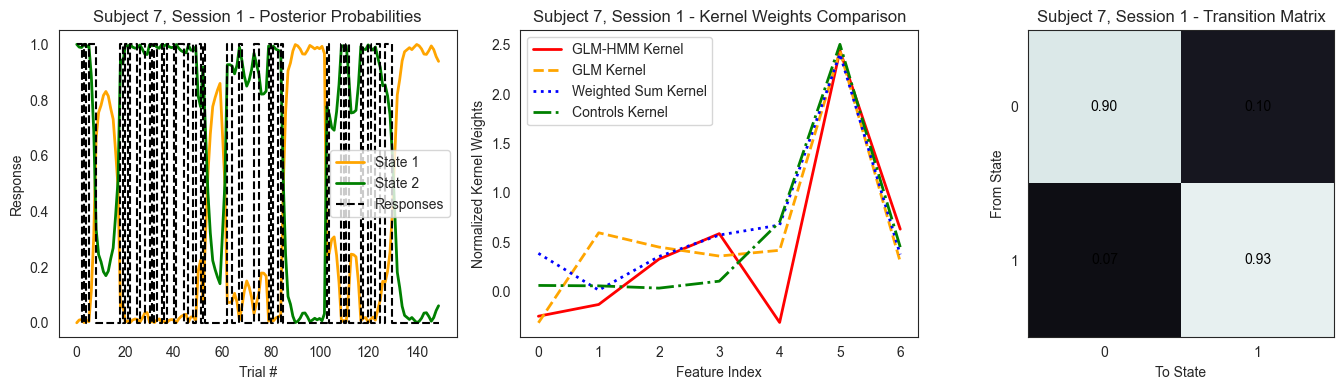
\includegraphics[width=16cm]{MainLayout/Images/chapter7/control.png}
    \caption{Main Title for First Image \\ \small Subtitle for the first graphic.}
    \label{fig:patient_responses}
\end{figure}
\subsection{Precision of kernel in engaged state}
\subsection{Precision of internal noise in engaged state}

\section {Dynamical GLM} 

\section {Discussion} 